\documentclass{beamer}
\usetheme[hideothersubsections]{HRTheme}
\usepackage{beamerthemeHRTheme}
\usepackage{graphicx}
\usepackage[space]{grffile}
\usepackage{listings}
\lstset{language=SQL,
basicstyle=\ttfamily\footnotesize,
mathescape=true,
keywordstyle=\color{blue},
breaklines=true
showstringspaces=false}
\usepackage[utf8]{inputenc}
\usepackage{color}
%\usepackage{wrapfig}
\newcommand{\red}[1]{
\textcolor{red}{#1}
}
\newcommand{\ts}{\textbackslash}
\newcommand{\valseq}[1]{$\lbrace$ #1 $\rbrace$}
\newcommand{\tuple}[2]{$t_{#1}$[#2]}
\newcommand{\fdep}[2]{#1 $\rightarrow$ #2}

\title{Data Source Architecture Pattern}

\author{TEAM INFDEV}

\institute{Hogeschool Rotterdam \\ 
	Rotterdam, Netherlands}

\date{}

\begin{document}
\maketitle

\SlideSection{Lesson 2 extra overview overview}

\begin{frame}
	\frametitle{Lesson topics}
	\begin{itemize}
		\item Impedance Mismatch
		\item Object Relational mapping
		\item Table Data Gateway
		\item Row Data Gateway
		\item Active Record
		\item Data Mapper
	\end{itemize}
\end{frame}

\SlideSection{Design Pattern}

\begin{frame}
	\frametitle{Motivation}
	\begin{itemize}
	\item Software systems may require persistent data (i.e. data 	that persists between program executions).
	\item In general, distributing low-level data access logic throughout a program is not a good idea (design).
	\end{itemize}
\end{frame}	
	
\begin{frame}
	\frametitle{Data Access Layer}
	\begin{itemize}
	\item A better design for your application is one that includes a data access layer which encapsulates the details of the underlying persistence.
	\item This layer must abstracts the low-level details of persistent storage.
	\item It also provides an interface that is usually a better match for the style of programming used in the domain logic. For example, the data access layer might provide an OO interface onto relational data.
	\end{itemize}
	\begin{figure}
	%	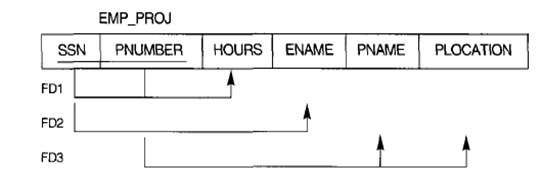
\includegraphics[scale=0.5]{img/normalization/norm15}
	\end{figure}
\end{frame}	

\begin{frame}
	\frametitle{Impedance Mismatch}
	\begin{itemize}
	\item There are a set of difficulties that are common when implementing a data access layer:
	\begin{itemize}
		\item Object-oriented concepts such as encapsulation, access modifiers and inheritance cannot sometimes directly be mapped or supported by RDBMS 
		\pause
		\item Data type differences between programming languages  and databases. For instance a string and the different type of collations in RDBMS. 
		\pause
		\item Structural and integrity differences. Data in one table are structured as tubles and organized the same way as the header. Using constrains in RDBMS helps to avoid data inconsistency. In your application it's not an easy task to implement such a constraint. You can use exceptions for instance to imitate the behavoir of some constraints  but not all of them.
	\end{itemize}
\end{itemize}
\end{frame}	

\begin{frame}
	\frametitle{Object Relational Mapping (ORM)}
	\begin{itemize}
	\item ORM is a programming technique for converting data between incompatible type systems in object-oriented programming languages. 
	\item Hides details of SQL queries from OO logic.
	\pause 
	\item Portability: DB independent
	\pause 
\end{itemize}
\end{frame}	

\end{document}

\begin{slide}{
\item ...
}\end{slide}

\begin{frame}[fragile]
\begin{lstlisting}
...
\end{lstlisting}
\end{frame}
